\documentclass[a4paper,8pt]{article}
\usepackage[utf8x]{inputenc}
\usepackage{graphicx}
\usepackage{listings}
%opening
\title{Teoría de Lenguajes\\ \textbf{TP2: “Micro HTML Prettyprint - segunda parte”}}
\author{1º Cuatrimestre 2013} 
\date{}


\begin{document}

\maketitle

\begin{center}
\vspace{10cm}

\begin{tabular}{|c|c|}
\hline
\hline
\textbf{Nombre}&\textbf{email}\\
\hline
\hline
Pablo Romano&pabloromano@gmail.com\\
\hline
Paula Verghelet (LU:836/02)&pverghelet@gmail.com\\
\hline
\hline
\end{tabular}
\begin{figure}[h!]
 \centering
 \includegraphics[scale=0.70]{logoDC.jpg}
 % logoDC.jpg: 321x144 pixel, 72dpi, 11.32x5.08 cm, bb=0 0 321 144
\end{figure}
\end{center}
\begin{section}{Introducción}
Como se describe en el enunciado, HTML es un lenguaje de marcado utilizado en la mayoría del contenido de la World Wide Web.
Muchos de los tags que conforman HTML son interpretados por los browsers para permitir la visualización de contenido de manera amigable (human readable). 

Se pide realizar un parser que interprete la estructura de los archivos HTML y que genere otro documento HTML que permita visualizar el HTML original de manera elegante (Prettyprint). Ciertos tags se verán de manera anidada mediante la indentación y los comentarios, tags, atributos y otros elementos de control se verán con diferentes colores (ver ejemplo en la figura 1).

\begin{figure}[h!]
  \centering
  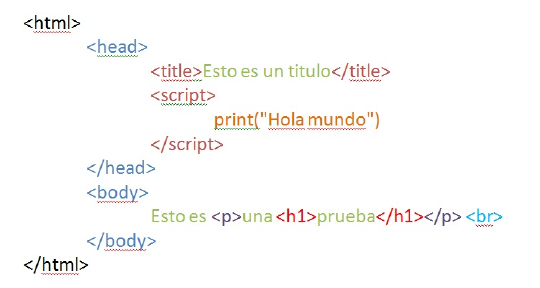
\includegraphics[scale=0.70]{salida.png}
  \caption{\texttt{Salida esperada para el siguiente HTML ``$<html> <head><title>Esto es un titulo</title> <!– esto es un comentario –> <script> print(”Hola mundo”)</script></head> <body> Esto es <p>una <h1>prueba</h1></p> <br></body></html>$''}}
\end{figure}

El trabajo práctico fue dividido en dos partes, la primera consistió en identificar cuál seria la gramática y los componentes léxicos de nuestro lenguaje y la segunda parte consiste en realizar el parser junto con las reglas semánticas que permitirán generar el HTML resultante.
 


\end{section}
\newpage
\begin{section}{Gramática}
\begin{subsection}{Descripción del HTML reducido a identificar}
Para simplificar el lenguaje, ya que HTML es muy completo y extenso, sólo se considerará un subconjunto de tags válidos, no se permitirán atributos y se espera que todos los tags tengan su tag de cierre correspondiente (salvo $<br>$).\\


Los tags que se considerarán son:

\textbf{$<html>-<head>-<body>-<title>-<script>-<div>-<h1>-<p>-<br>$}.\\

Con las siguiente restricciones:

\begin{itemize}
 \item Es obligatorio que el documento completo esté rodeado por tags de apertura y cierre $<html>$
\item dentro del html puede tener una sección opcional $<head>$ y otra sección también opcional $<body>$
\item dentro de la sección head pueden aparecer indistintamente y en orden no preestablecido secciones $<title>$ y $<script>$
\item $<title>$ contiene texto sin tags
\item dentro de la sección $<script>$ puede haber cualquier cosa salvo el tag de cierre de dicha sección
\item dentro de la seccion $<body>$ tendremos bloques de texto con subsecciones (div, h1 o p) o con tags $<br>$ sueltos, las subsecciones se comportan como la sección $<body>$
\end{itemize}


\end{subsection}

\begin{subsection}{Gramática utilizada para la primera parte del tp}
\bigskip

\begin{verbatim}
S -> E<html>EAE</html>E | E<html>ECE</html>E | E<html>E</html>E
A -> <head>EBE</head>ECE
B -> <title>T</title>EBE | <script>T</script>EBE | lambda
C -> <body>EDE</body> | <body>TDT</body>  | lambda
D -> T D | lambda | <div>EDE</div>EDE | <p>EDE</p> EDE | <h1>EDE</h1> EDE |
    |<br>EDE | <div>TDT</div>TDT | <p>TDT</p>TDT | <h1>TDT</h1>TDT | <br>TDT
E -> espacioE | E<!–-T-–>E  | lambda 
T -> (a|...|z|A|...|Z|0|...|9|...|&|;|espacio|... )T | E |lambda  
espacio pertenece a {“ “}

\end{verbatim}
\bigskip

Descripción de la gramática
\begin{enumerate}
 \item Todas las derivaciones del símbolo distinguido comienzan (terminan) con cero o más espacios y luego un tag de apertura (cierre) de html, la derivación que contiene A corresponde a un HTML con head mientras que la que contiene C es un HTML que no tiene head
 \item La derivación de A corresponde a un head seguido de cero o más espacios, cero o un body y cero o más espacios
\item La derivación de B es el contenido que puede estar dentro de un head, estos son titles (conteniendo texto) o scripts (conteniendo texto), en ambos casos puede haber cero o más ocurrencias
\item La derivación de C permite que haya cero o un body conteniendo tags, ver EDE y TDT en el punto siguiente.
\item Derivaciones de D: a) TD  , esto permite agregar texto a izquierda de los tags, como el tag puede derivar en $\lambda$ esto también permite terminar con texto a derecha “quitando” el último D - b) Las derivaciones rodeades de div, p y h1 permiten generar estos tags, en todos los casos contienen EDE que permite nuevos tags rodeados de cero o más espacios o derivar D a TD y generar texto - c) La derivación $<br>EDE$ permite generar el tag $<br>$ - d) Las derivaciones que contienen TDT son todas redundantes por lo expuesto en 5.a y 5.b pero hacen que los ejemplos sean más compactos
\item Esta derivación permite generar cero o más espacios o comentarios
\item Esta derivación permite generar texto de longitud cero o mayor, se agregan los símbolos $\&$ y $;$ para poder codificar las entidades html y se permite derivar a E para poder incluir comentarios ya que esto siempre es válido
\end{enumerate}

\end{subsection}

\begin{subsection}{Gramática corregida}
En las correcciones se nos indicó que devíamos completar los tokens léxicos para los tags y definir correctamente el conjunto de terminales para el texto.
\bigskip

\begin{verbatim}
S -> E I_HTML EAE F_HTML E | E I_HTML ECE F_HTML E | E I_HTML E F_HTML E
A -> I_HTML EBE F_HTML ECE
B -> I_TITLE T F_TITLE EBE | I_SCRIPT T F_SCRIPT EBE | lambda
C -> I_BODY EDE F_BODY | I_BODY TDT F_BODY  | lambda
D -> T D | lambda | I_DIV EDE F_DIV EDE | I_P EDE F_P EDE | 
     | I_H1 EDE F_H1 EDE | I_BR EDE | I_DIV TDT F_DIV TDT | 
     | I_P TDT F_P TDT | I_H1 TDT F_H1 TDT | I_BR TDT
E -> espacioE | E I_COMMENT T I_COMMENT E  | lambda 
T -> TEXTO_SIN_TAGS 
espacio pertenece a {' '}

---------------- TOKENS LEXICOS ---------------------------
I_HTML 	:	'<html>' 
F_HTML 	:	'</html>' 

I_HEAD 	:	'<head>'  
F_HEAD 	:	'</head>' 

I_BODY 	:	'<body>' 
F_BODY 	:	'</body>'

I_TITLE:	'<title>'  
F_TITLE:	'</title>' 
	
I_SCRIPT:	'<script>'  
F_SCRIPT:	'</script>' 
	
I_DIV 	:	'<div>' 
F_DIV 	:	'</div>' 
	
I_H1 	:	'<h1>'  
F_H1 	:	'</h1>' 
	
I_P 	:	'<p>'
F_P 	:	'</p>' 

BR 	:	'<br>'

I_COMMENT:	'<!–-'
F_COMMENT:	'-->'

TEXTO_SIN_TAGS 
	:	(~('<' | '>' | '\t' | '\r'| '\n'))* 

WS 
    :   ('\t' | '\r'| '\n') 

\end{verbatim}
\bigskip
\newpage
 \begin{subsubsection}{Arboles de derivación - Ejemplos}
    \begin{figure}[h!]
      \centering
      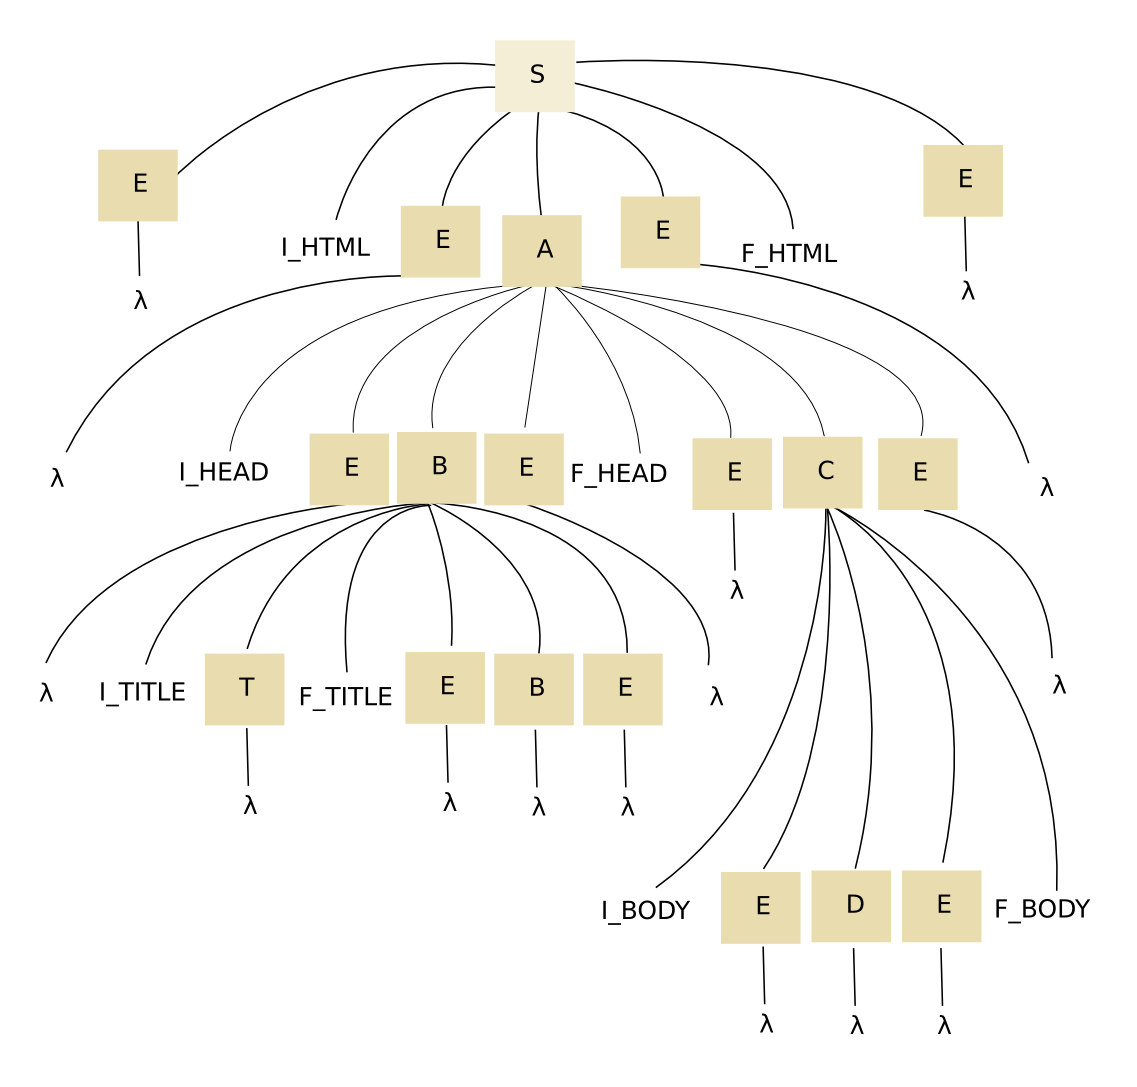
\includegraphics[scale=0.40]{ejemplo1.png}

      \caption{Arbol de derivación para ``$<html><head><title></title></head><body></body></html>$''}
    \end{figure}

 \end{subsubsection}

\end{subsection}
\newpage

\begin{subsection}{Gramática modificada para la segunda parte del tp}
Una vez definida la gramática, en esta segunda parte, se construye el parser y se agregan reglas semánticas que permitan:\\
\begin{itemize}
 \item La salida será un documento que se visualice desde un browser como código HTML (Figura 1).
\item El código del HTML de entrada deberá aparecer formateado con cada línea indentada según el nivel de anidación del código del archivo HTML de origen. 
\item A cada clase de token se le deben poder asignar distintos atributos visuales. En cuanto a los atributos visuales, se requiere un color para los tags head y body, otro para los tags title y script, otro para el tag h1, otro para el tag div y otro para el tag br. Otro color para el texto y otro para los scripts.
Se sugiere que cada token quede incluido en un elemento de tipo SPAN que indique de qué clase es.
Por ejemplo:$<SPAN class=``tagH1''>\&lt;h1\&gt;</SPAN>.$

\end{itemize}

La gramática fue transformada en una $ELL(1)$ ...

\textbf{(COMPLETAR)}
\bigskip

\begin{verbatim}
  
------------------ GRAMATICA -----------------------------
public html 	:	I_HTML head? body? F_HTML;

head 	:	I_HEAD (title | script)* F_HEAD;

title 	:	I_TITLE TEXTO_SIN_TAGS? F_TITLE;
script 	:	I_SCRIPT TEXTO_SIN_TAGS? F_SCRIPT;

body 	:	I_BODY tags F_BODY;

tags	:	TEXTO_SIN_TAGS? tag*;

tag	:	(I_DIV tags F_DIV | I_H1 tags F_H1 | I_P tags F_P | BR) TEXTO_SIN_TAGS?;


---------------- TOKENS LEXICOS ---------------------------
I_HTML 	:	'<html>' { ImprimirTag("html", true); };
F_HTML 	:	'</html>' { ImprimirTag("html", false); };

I_HEAD 	:	'<head>'  { ImprimirTag("head", true); };
F_HEAD 	:	'</head>' { ImprimirTag("head", false); };

I_BODY 	:	'<body>'  { ImprimirTag("body", true); };
F_BODY 	:	'</body>' { ImprimirTag("body", false); };

I_TITLE
 	:	'<title>'  { ImprimirTag("title", true); };
F_TITLE 
	:	'</title>' { ImprimirTag("title", false); };
	
I_SCRIPT
 	:	'<script>'  { ImprimirTag("script", true); };
F_SCRIPT 
	:	'</script>' { ImprimirTag("script", false); };
	
I_DIV 	:	'<div>'  { ImprimirTag("div", true); };
F_DIV 	:	'</div>' { ImprimirTag("div", false); };
	
I_H1 	:	'<h1>'  { ImprimirTag("h1", true); };
F_H1 	:	'</h1>' { ImprimirTag("h1", false); };
	
I_P 	:	'<p>' { ImprimirTag("p", true); };
F_P 	:	'</p>' { ImprimirTag("p", false); };

BR 	:	'<br>' { ImprimirTag("br", null); };


COMENTARIO 
	:	'<!--' TEXTO_SIN_TAGS '-->' {$channel=HIDDEN;};

TEXTO_SIN_TAGS 
	:	(~('<' | '>' | '\t' | '\r'| '\n'))+ { Console.WriteLine(Text); };
	
WS 
    :   ('\t' | '\r'| '\n') {$channel=HIDDEN;}
    ;

 \end{verbatim} 

 \begin{subsubsection}{Ejemplos}
  
 \end{subsubsection}

\end{subsection}
\end{section}
\newpage
\begin{section}{Implementación}
\begin{subsection}{Discusión}
%Descripción y decisiones tomadas
\end{subsection}
\begin{subsection}{Resultados}

\end{subsection}
\begin{subsection}{Ejemplos de uso}

\end{subsection}
\begin{subsection}{Código Fuente}

\end{subsection}
\end{section}
\newpage
\begin{section}{Conclusiones}
 
\end{section}
\newpage

\end{document}
